\documentclass[11pt]{article}
\usepackage{a4wide, graphicx, fancyhdr, wrapfig, tabularx, amsmath, amssymb, hyperref, color, verbatim, nameref}
\usepackage[english]{babel}
\definecolor{linkcolour}{rgb}{0,0.2,0.6}
\hypersetup{colorlinks,breaklinks,urlcolor=linkcolour, linkcolor=linkcolour}

%----------------------- Macros and Definitions --------------------------

\setlength\headheight{20pt}\usepackage{}
\addtolength\topmargin{-10pt}
%\addtolength\footskip{20pt}

\fancypagestyle{plain}{%
\fancyhf{}
\fancyfoot[RO,LE]{\sffamily\bfseries\thepage}
\renewcommand{\headrulewidth}{0pt}
\renewcommand{\footrulewidth}{0pt}
}

\pagestyle{fancy}
\fancyhf{}
\fancyfoot[RO,LE]{\sffamily\bfseries\thepage}
\fancyhead[RO,LE]{\textsc{}}
\fancyhead[LO,RE]{\emph{}}
\renewcommand{\headrulewidth}{1pt}
\renewcommand{\footrulewidth}{0pt}
\newcommand{\tab}{\hspace*{2em}}

\newcommand{\tocheck}[1]{{\bf !?: #1 :!?}}
%\newcommand{\OBA}{Online behavioural advertising }

\frenchspacing

\usepackage{booktabs}
\usepackage[parfill]{parskip}
%-------------------------------- Title ----------------------------------

\title{\textbf{Honeypot Assignment: \\ \emph{Group Contagiarium}}}
\author{Aram Verstegen, s4092368 \\
	 Mark Vijfvinkel, 1275194 \\
	 Bart Lutgens, 12752408 \\
	Joost Kremers, 1275259}

\date{\today}

\begin{document}
\maketitle


\section{Introduction}
\tocheck{Kijken of the secties nog kloppen!}
In this paper we will try to present an overview of the data we have collected from the honeypot and explain the different attacks that were waged against it. 
In the second section we will describe the changes we have made to the setup during the "Waiting for hackers" phase. 
The third section will present an overview of various statistics we have collected from the logfiles, e.g. number of IP-addresses, countries and attack types. 
In the fourth section we will discuss which attacks took place against the different services the honeypot was running e.g. SSH and MySQL.
In order to discover the sophisticationof the attacks, we will try to present possible connections between an attack on one service and an attack on a different service, in the fifth section.
The sixth section will conclude our findings. 
Finally we will discuss this project and provide some improvements. 


\section{Setup}
\label{Setup}

On the 1st of November we delivered our initial setup document, however during the "Waiting for hackers" phase we have made adjustments to the setup in order to attract more activity to the honeypot. In this section we will present the initial setup and in addittion to that, discuss the changes that were made.

%%%%MOET NOG WORDEN HERZIEN%%%%%

\subsection{Rsyslog}
At first the rsyslog configuration was stored in its own file in the syslog.d directory, which might have been seen by an attacker.
Therefore we have moved it to the default syslog configuration file. 

\subsubsection{Kippo}
During the second phase of the project, we noticed that of the succesful dictionary-based bruteforce attempts against Kippo, none actually tried to continue and explore or use the honeypot.
Running an nmap portscan from Metasploit (which adds to the information provided by nmap) revealed that it can detect if Kippo is being used.
This doesn't explain why people should refrain from logging in after a successful dictionary attack

\subsubsection{DenyHosts}
If someone found out that our real SSH port was changed to 9022, they might try to break in through the real SSH service.
To make sure no bruteforce attacks could be done on this port, DenyHosts was installed.
This service blocks IP-addresses that try to log in more than 3 times with the wrong password by adding them to the \verb|hosts.deny| file.
The hosts listed there are blacklisted on the machine, but we can edit them if needed.

%Denyhosts can log to syslog by editing its configuration file.

\subsection{Apache \& Nginx}
To attract web traffic, we installed the Apache web server, the Apache PHP runtime and the \verb|mod-security| module which allows us to spoof its version information, to make it appear old and vulnerable.
The Nginx webserver is installed as a reverse proxy in front of Apache, which runs on local port 8080.
This provides 2 layers of logging (to files), and Nginx's superior transparent caching mechanism allows us to avoid exhausting our resources with scripting languages, should we have ever faced an application-layer DoS attack (Nginx appears quite resilient against those).

Nginx has been compiled from source and was patched to send the spoofed Apache version header as well.
We will configure both services to log to our \verb|sshfs| mount.

\subsubsection{Google Hack Honeypot}
Google Hack Honeypot (GHH) is designed to be used to attract search engine attackers. 
These attackers will use search queries to find sensitive data, for example password files, that due to some misconfiguration ended up being indexed by a search engine like Google.
GHH allows logging of these requests to a MySQL database or Comma Seperated Value (CSV) file.

Since GHH offers multiple search targets, we picked one to start with, namely GGH version 1.2 passlist.txt.
We had no particular reason for this, only that it was easy to set up. 
%We plan to install more variants of the GHH to attract more attackers, but before this could happen the VM's were shut down.

%To set up GHH we have first installed Apache and PHP5.
We configured GHH to log to in CSV format, since it requires minimal setup and is easily parsed.
%We can later reconfigure to use MySQL, if the results are not satisfactory.
Then, we patched the GHH code to allow logging to syslog, to maintain a single, consistent point of log collection.

We hoped to detect and capture a bruteforce attack or scan on generic filenames, for example \verb|passwd.txt|, because this would probably have warned us that an attacker will try to use a dictionary attack.
Unfortunately GGH broke down after the Virtual Machines were shut down, we were unable to get it back up running and therefore decided not invest more time and effort into it. We also believe it would not have brought us more interesting data.

\subsubsection{Website}
To attract more activity we decided to create a fake website that would resemble a website of the University of Twente. To make it more appealing in ways of computing power we used the department of Partical Physics and Astronomy as a cover.
On the website we also put some information about a fictive person (Jenny Abott) would manage the servers and website. So we created a useraccount with the same login and password, namely Jenny. This way a more sophisticated attack would be possible. An attacker would look at the website, determine if it is intresing to attack and then connect to Kippo to log in as Jenny.

\subsubsection{Wordpress}
In order to make the website more vunerable and appealing to hackers, we installed an out of date version of Wordpress. Wordpress is software, powered by PHP and MySQL, that can be used to easily create websites or blogs and manage them via the content management system. Exploits are found on a frequent basis for Wordpress and therefore patches are published frequently. In the first week of December we installed version 2.8.4 of Wordpress on the honeypot.

\subsubsection{Snort and Suricata}
Snort is an open source intrusion detection system (IDS) that uses realtime traffic analysis and packet logging on internet protocol networks.
Snort was designed to be used as a network IDS, however we will be running it on our host machine, effectively making it a host-based IDS.

We set up Snor using the community rule-set that will only alert on suspicious network behaviour, but do nothing to prevent it. 
Included are rules on detecting exploit attempts on various common services like HTTP, FTP, SMTP, and many more.

We configured Snort to send alerts to syslog, and to log its packet captures to the read-only \verb|sshfs| mounted from our monitoring machine.
We also installed \verb|oinkmaster| to automatically retrieve the latest community Snort rules, with a Snort API key registered specifically for this project.

Unfortunately we noticed that Snort required a lot of resources and was slowing down the honeypot. Instead of Snort we decided to use Suricata, which uses the same ruleset, but uses it more efficiently and therefore less resources.

\subsubsection{Dionaea}
Dionaea is a low interaction honeypot that provides several services, namely http, ftp, tftp, MSSQL, MySQL and SIP (VoIP). We installed this to enable more services and attract more traffic to the honeypot. 

%Considering we are in a VM we might be limited in RAM, which Snort seems to require a lot of.
%The configured rules will have to be minimal to avoid exhausting resources.

\subsubsection{Auditing}
During the High Interaction phase we used a kernel module that hooked execve (new process) calls and commandline interaction. This information was logged to syslog which provided us with auditing information during this phase.
%For the HI phase, we would like to have a way to audit commandline interaction. 
%Various options exist, such as the user-space \verb|auditd| daemon, but to make auditing harder to detect this we feel it would be best to look for a kernel-space solution.
%An auditing module developed by the Honeynet project called Sebek can provide this, but is unmaintained and outdated.
%The grsec kernel patches also provide auditing from kernel space, but we were advised against replacing the stock kernel.

%We are still investigating the best way to achieve useful auditing.
%A self-written kernel module that hooks system calls, albeit limited, might suffice to get some much needed auditing information from the honeypot.


\section{Statistics}
\label{Statistics}
In this section we will discuss the statistical data that have been gathered from our logfiles. 
The logged connection attempts have been processed to group them by the IP address' originating country through the use of WHOIS directory service information.
It is worthwhile noting that a significant number of connecting hosts could not be referenced to RWHOIS information.
In these cases we have attempted to resolve the missing information by making use of reverse DNS queries and grouping by associated top level domain.
Also note that these graphs display all logged connection attempts rather than successful connections, giving us a general view of which ports attract attention.

For clarity we have chosen to graph only the 10 most active originating countries, and make use of a logarithmic scale to represent the spectrum of port numbers.
The labels on the \(y\)-axis were chosen based on the most frequently accessed ports, with some selected labels removed to avoid clutter.

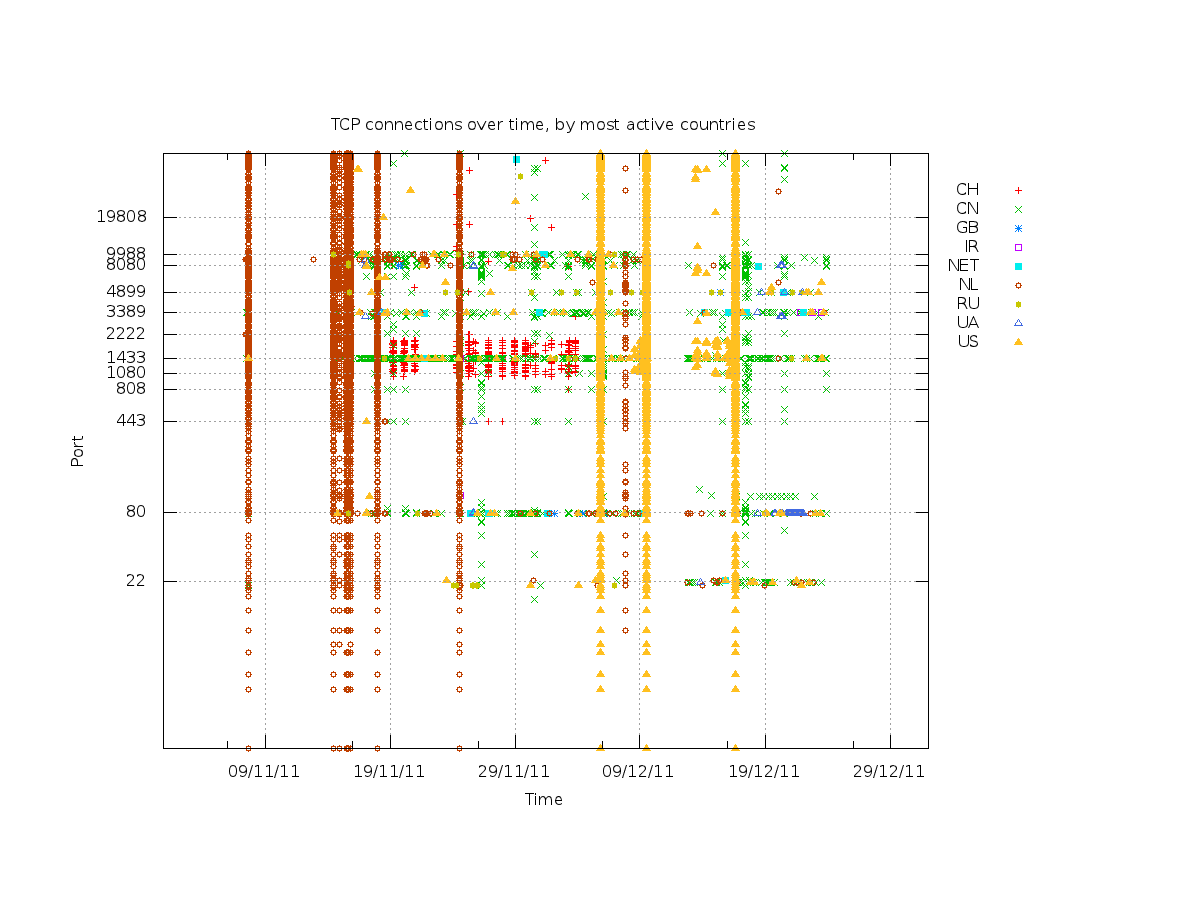
\includegraphics[width=1.7\textwidth,angle=-90]{tcp.png}

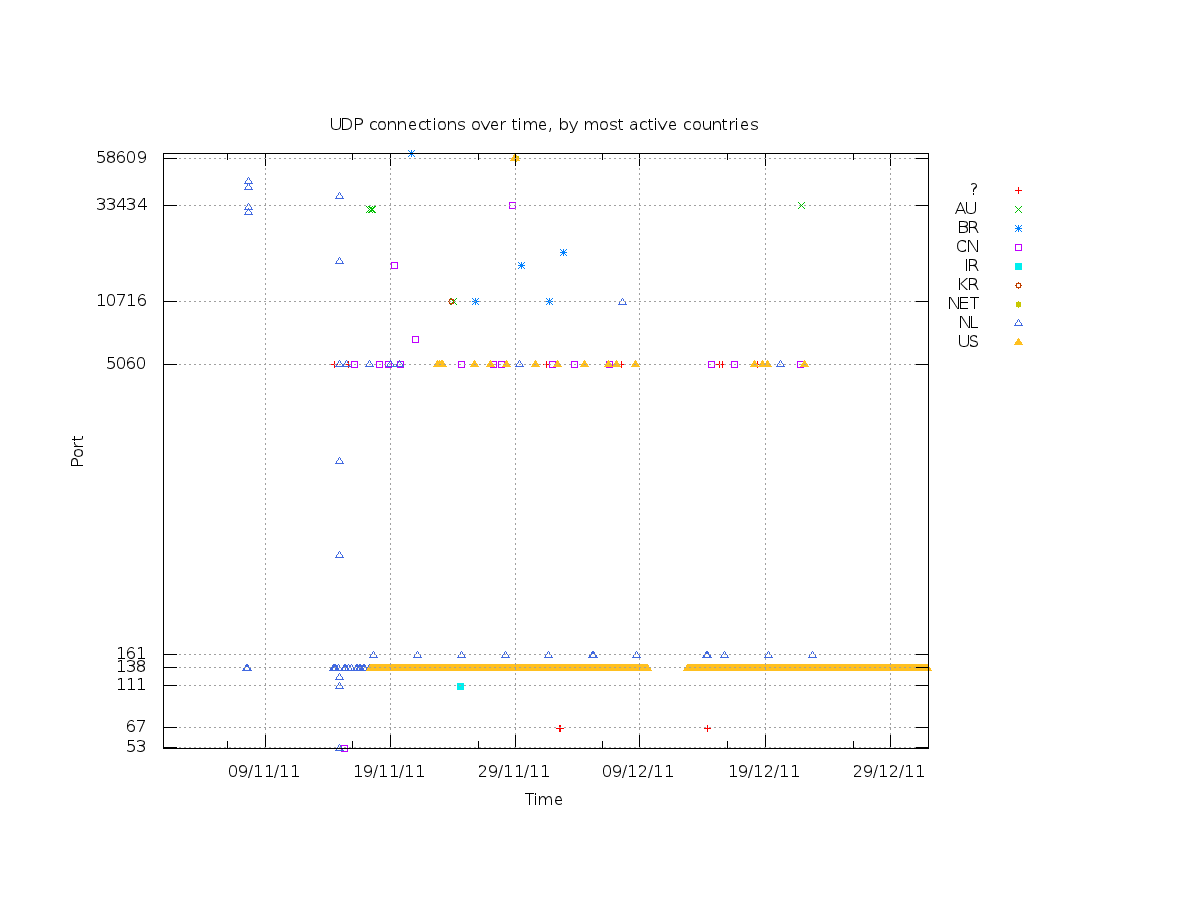
\includegraphics[width=1.7\textwidth,angle=-90]{udp.png}

\section{Attacks on the different services}
\label{Attacks}
During phase 2 we have monitored the honeypot closely and collected data about different attacks against the honeypot. In this section we will discuss the attacks against the services the honeypot was running.

\subsection{Kippo}

The first service we will be talking about is Kippo. During the interaction phase we've had 2610 login attempt on our Kippo client and 3871 connections. 54 of these attempts were successful.
We have made a top 5 of most tried usernames in these login attempts:

\begin{tabular}{|l|r|}
\hline
Username & Attempts \\ \hline
root & 2206 \\ \hline
admin & 39 \\ \hline
bin & 26 \\ \hline
w000t & 20 \\ \hline
oracle & 19 \\ \hline
jenny & 19 \\ \hline
\end{tabular}

It is not entirely unexpected that the username ``root'' is tried most often. 
The username ``w000t'' is a backdoor user created in the FAKE Apache 2.2.17 exploit.
Interesting to note is that ``jenny'' is the name of a fake employee listed on the our honeypot website.
Most usernames were tried multiple times, even if they made no sense to us for instance ``msnayeem\_iitd'' tried to log in four times.

These are the top 5 passwords tried:

\begin{tabular}{|l|r|}
\hline
Password & Attempts \\ \hline
  & 55 \\ \hline
123456 & 28 \\ \hline
111111 & 20 \\ \hline
root & 16 \\ \hline
admin & 16 \\ \hline
\end{tabular}

As you can see, the most tried password is a blank password. The other passwords in this top 5 are all standard password that can be found in a dictionary attack. It is nice to note that 123456 was accepted by our system.

An interesting situation was someone that tried to log in to the honeypot with the user root, just trying a list of years (1960-1980). It seems like an unusual brute force attack. Assuming someone used their birthday as a password, which still happens a lot, it is unlikely that this someone just used their birth year and not the whole birthday. However brute forcing for the entire birthday takes way to long. So for a quick and easy brute force it is unlikely to yield results.

\subsection{HTTP}
In three weeks, a total of 76002 HTTP-requests were received by our Apache server originating from 176 unique IP addresses. 4369 of these requests were 404'd.

These 404's are interesting because they show us what addresses the attackers were trying to access. For instance, we see a lot of scans for phpMyAdmin (phpMyAdmin-3.3.10.5, phpMyAdmin-3.4.7, phpMyAdmin-3.4.6 etcetera). They also searched non existing folders for these phpMyAdmin files. 

Also several client IDs are visible in these logs: 

\begin{itemize}
\item \emph{``-''} (3432 attempts)

This is a blank user/client ID. Which seems to be a popular client to use when you want to find weak software on a server.

\item ``MiRRORS'' (310 attempts)

Due to the well-chosen name we could not find additional information on this client. Mirrors is a frequently used word on the internet.

\item ``ZmEu'' (41 attempts)

The attackers using ``ZmEu'' found one valid path: /phpmyadmin/, however he did not exploit this. 
It is interesting to see that both several \emph{''-''} and several ``ZmEu'' users are scanning for ``/w00tw00t.at.blackhats.romanian.anti-sec:)'' and ``/w00tw00t.at.ISC.SANS.DFind:)'' These clients are alleged to be for reconnacance purposes.

\item ``Morfeus Fucking Scanner'' (4 attempts)

``Morfeus Fucking Scanner'' was used by one attacker, that solely searched for /user/soapCaller.bs. Multiple sources say this might be a Drupal exploit.
\end{itemize}

We expected to see several occurrences of ``/robots.txt'' because this is a common way to start when using a search engine crawler, but none were found.

\subsection{Dionaea}
As mentioned in Section \ref{Setup} Dionaea runs several services. In the table below we will show how many times those services got connected.

\begin{tabular}{|l|c|r|}
\hline
Service & Port & Number of connections \\ \hline
MSSQL  & 1433 & 1632 \\ \hline
MS SMB filesharing & 445 & 67 \\ \hline
FTP & 21 & 55 \\ \hline
MySQL & 3306 & 54 \\ \hline
Session Initiation Protocol & 5060 & 9 \\ \hline
\end{tabular}

As we looked further into the Dionaea logfiles we found that MSSQL was connected to from 95.82.11.28, which is in Iran, 1414 times. However, the SMB filesharing, FTP and SIP were mostly connected from one IP, namely 130.89.165.58. This IP is from Twente University, so probably it was another student.




\section{Connection between the attacks}
\label{Connection}
In this section we will correlate the data about attacks against one service against the data of attacks of a different service. We will try to look for a pattern or similarities in this data and determine if the attack was more sophisticated.

Three clients connected to both HTTP and Kippo, which raised our suspision:
\begin{itemize}
\item 58.17.52.14

This citizen of the Peoples Republic of China poked every possible entrance, in two consequental days: he made a connection to Kippo and disconnected immideately. He also requested the main / folder via HTTP, using the client "-". Scanlogd also reported scans on port 80, 8080, 3128, 9415, 8909, 9592, 1080, 443. Unfortunately for us we were not attractive for him to return and actually break in.

\item 61.190.172.2

On four occasions this inhabitant of China probed us, split over 4 weeks. He also just connected to Kippo (Suricata reported a SSH-scan) and disconnected: he did this for fourty times in 3 minutes. Interestingly enough he was one of the users of the Morfius Fucking Scanner client: only requesting the /user/soapCaller.bs file.

\item 125.88.75.199

The last prober was also from China. On November 22th he connected to Kippo to automaticly disconnect again. He also requested the / folder via HTTP with the "-" client. He was only seen at this occasion.

\end{itemize}


\section{Conclusion}
\label{Conclusion}
From Section \ref{Attacks} we can conclude that our honeypot was not as popular as we had hoped it would be. Because we chose not to advertise, we solely relied on the hackers abilities to find us by for example portscans. The number of attacks on us was therefore not high and neither was the depth of the attacks. 

Concluding: 


\section{Discussion}
\label{Discussion}
In this section we would like to discuss some issues we encountered during the honeypotproject. 

\begin{itemize}
\item Low/High interaction phase

To see what the best approach is to a honeypot project, we decided to split the project in a Low and a High interaction phase. Unfortunately the High interaction phase yielded not much more results than the low interaction phase. Additionally we were a little late in switching to the HI phase. So in hindsight we don't think it was worth switching to the high interaction phase.

\item Lack of interest

We decided to make this honeypot as realistic as possible, this meant: not advertising our honeypot on IRC-channels or 4Chan. Our motivation was that in nonhoneypot circumstances this would also not be done. So for example advertising the IP address of the honeypot would attract a lot more hackers than a normal server would. So the results would not be on par with attacks against a normal server. In the High interaction phase we had a website that attracted people to our honeypot, which is a more realistic approach to attracting hackers.

\item DenyHosts

To make sure our real SSH port would not be brute forced, we added DenyHost to the port. We soon realized that this was a very effective countermeasurement versus intruders: both Bart and Joost were blocked due to their lack of Linux knowledge. Luckely Mark and Aram were able to unblock the other two.

\item Linux knowledge

Two of the teammembers had limited Linux experience. It took some time for them to understand how Linux commandline works. Fortunately we had two guru's in the group that were able to teach the newbies.

\item Google Hack Honeypot

The Google Hack Honeypot was supposed to attract hackers. Unfortunately it soon crashed due to unknown configuration errors. Because the results in the period the tool was running were nonexistent and we were switching to HI later on, we decided not to use it. 

\end{itemize}

%%% REFS %%%

\bibliographystyle{plain} % amsalpha
\bibliography{ref_honeypot}

\end{document}
